\documentclass[letterpaper,titlepage,12pt]{article}
\author{Ashley Towne}
\title{Semiclassical Analysis of Quantum Mechanical Calculations of Rotational
Inelastic Collisions of He and Ar with NaK}
\pagestyle{plain}
\usepackage{graphicx}
\usepackage{amsmath}
\usepackage{epstopdf}

\begin{document}
\maketitle
\tableofcontents

\newpage
\section{Abstract}

\newpage
\section{Introduction}
NaK, like any molecule, can vibrate and rotate and can be described by its
rotational and vibrational states.  Upon collision with a perturbing atom,
such as helium or argon, these states can change.  This project was primarily
concerned with collisions where the vibrational state is conserved, but the
rotational state is not, as equation~\ref{eq:collisions} specifies.  
\begin{eqnarray}
    He+NaK(v,m,j)&\rightarrow& He+NaK(v,m',j') \nonumber\\
    Ar+NaK(v,m,j)&\rightarrow& Ar+NaK(v,m',j')
    \label{eq:collisions}
\end{eqnarray}
Specifically, the purpose of this investigation was
to explore the physical interpretations of how the quantum numbers that
describe angular momentum change during collision.

In addition to its rotational and vibrational states, NaK can also be described
by its electronic state, of which the set of potential curves are an
expression. A set of NaK's potential curves can be seen in
figure~\ref{fig:potentialcurves}. The potential curves represent energy as a function of internuclear
separation between sodium and potassium. Both experimental and theoretical
investigations choose one potential curve to study, specifying the electronic
energy level at which the collisions in question take place.

\begin{figure}[h]
    \centering
    \includegraphics[width=0.7\textwidth]{potentialcurves.eps}
    \caption{Potential curves for NaK}
\label{fig:potentialcurves}
\end{figure}
At Lehigh University, the experimental and theoretical investigations have
worked together to form a more complete picture of the collisions in question.
Professor Huennekens leads the experimental group, and Professor Hickman leads
the theory group.

\newpage
\section{Background}
\subsection{Experimental Measurements}
Professor Huennekens' experimental group has measured the rate constants (k) of
transitions, which are related to the cross sections.  The rate constants are
proportional to the expectation value of the product of the cross section and
velocity, which can be approximated as the cross sections times the average
velocity:
\begin{eqnarray}
    k&=&\langle\sigma v\rangle \nonumber\\
    k&\approx& \sigma \overline{v}
\end{eqnarray}
The cross section is a metric of the likelihood that a particular
transition will occur from one \(j\) state to another.  The rate constants average
over all values of the quantum number m.

The experimental group has also measured the fraction of orientation that is
preserved throughout the collisions.  Collisions tend to be randomizing processes, so
studying the extent to which orientation is preserved gives a metric of the
extent to which a particular type of collision is actually a randomizing
process.  In a cell environment, such as the system that the experimental group
studies, the angular momenta initially point in all directions and the average
value of \(m\) is zero.  In order to measure the change in orientation, the initial
orientation must be nonzero.  The orientation is proportional to the
expectation value of \(m\) for a particular \(j\) state:
\begin{equation}
    O^j={{\langle m\rangle}\over{\sqrt{j(j+1)}}}
    \label{eq:orientation}
\end{equation}
Physically, it is the extent to which all angular momenta point in the same direction.

\newpage
\subsection{Vector Model}
The orientation is  related to the geometric relationship between \(m\) and \(j\) in
the vector model, as seen in figure~\ref{fig:vectormodel}.
\begin{figure}[h!]
    \centering
    \includegraphics[width=0.5\textwidth]{vectormodel.eps}
    \caption{Vector model of angular momentum}
\label{fig:vectormodel}
\end{figure}
\newline
The vector model is a way of understanding angular momentum,
where \(j\) is the angular momentum vector.  The quantum number \(m\) is the
projection of \(j\) onto the z axis.  \(j\) can precess around the z axis at a constant
\(\theta\) without changing its magnitude or the magnitude of m, as stated by
equation~\ref{eq:vector_model_geometry}:
\begin{equation}
    \cos\theta={{m}\over{\sqrt{j(j+1)}}}
    \label{eq:vector_model_geometry}
\end{equation}
The expectation value of the \(\cos\theta\) is the orientation, as
equation~\ref{eq:orientation} stated.

\newpage
\subsection{Experimental Procedure}
In order to choose a nonzero orientation for the initial state of the system,
the experimental group excites the system from the ground state to a higher
potential, the A state.  These states are selected potential curves from
figure~\ref{fig:potentialcurves}, shown in more detail in
figure~\ref{fig:selected_potcurves}.  A pump laser that is left circularly polarized
populates the A state's vibrational and rotational states.  After the collisions, the probe laser is swept
across a range of frequencies to measure the orientation.
\begin{figure}[h]
    \centering
    \includegraphics[width=0.5\textwidth]{selected_potentialcurves.eps}
    \caption{States used in experiment. \(X^1\Sigma^+\) is the ground state,
    \(A^1\Sigma^+\) is the chosen excited state, and \(3^1\Pi\) is the state to
which the system is excited by the probe laser}
\label{fig:selected_potcurves}
\end{figure}

Polarized light always has selection rules for which states it populates, and
the circularly polarized pump laser's selection rule for \(\Delta m=+1\) leads to
a preferential population of large m.  This can be seen in
figure~\ref{fig:m_potcurves}.
\begin{figure}[h]
    \centering
    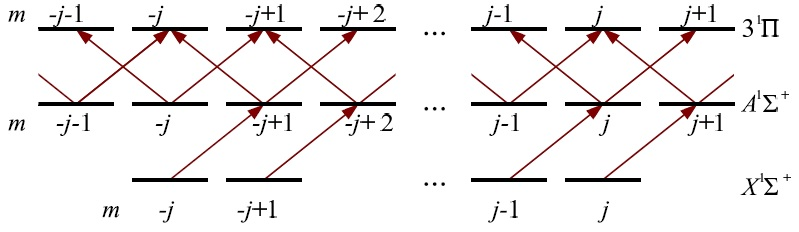
\includegraphics[width=1\textwidth]{m_potcurves.jpg}
    \caption{Bottom row: \(m\) states available in the ground state
        Middle row: \(m\) states available in the \(A^1\Sigma^+\) state
        Top row: \(m\) states available in the \(3^1\Pi\) state
    Arrows show possible transitions}
\label{fig:m_potcurves}
\end{figure}

The probe laser is linearly polarized; linear polarization can be expressed as
a superposition of left and right circularly polarized light.  Because of the
initial nonzero orientation of the system, the different circular polarizations
interact with the system differentially.  Essentially, the left circular
polarization will see a different system than the right circular polarization
because of the states occupied and available states for transition.  After
interacting with the sample, the superposition of light that was not absorbed is passed through a linear
polarizer perpendicular to the intial polarization.  If the laser is unchanged,
no signal will pass through the polarizer.  However, because the left and right
circular polarizations are absorbed differently, the superposition after
interacting with the system is no longer perfectly linear but rather
elliptically polarized.  Therefore, whatever signal is detected after the
polarizer is a metric of the final orientation.

\newpage
\subsection{Previous Results}
Experiment and theory tend to agree in their determinations of the rate
constants.  For helium, past work has shown that there is a propensity for the
change in \(j\) to be an even number. See figure~\ref{fig:He_past_results}.
\begin{figure}[h]
    \centering
    \textbf{Helium Rate Constant}\par\medskip
    \includegraphics{He_past_results.eps}
    \caption{Rate constants for helium vs. \(\Delta\)j (Malenda et al)}
\label{fig:He_past_results}
\end{figure}

It was originally thought that this propensity was related to the strict
selection rule for homonuclear diatomic molecules where no odd \(\Delta j\)
transitions are allowed.  Sodium and potassium are in the same column of the
periodic table, so it was thought that perhaps NaK was approximately
homonuclear, which would explain the propensity.  However, it has been
demonstrated that the propensity for an even \(\Delta j\) depends on the collision
partner, where as behavior of an approximately homonuclear molecule should
depend solely on the molecule.  Some initial experimental results for certain
states in a collision with potassium show no propensity for even \(\Delta j\) at
all.  Unfortunately, theory has large computational requirements, and it is too
computationally expensive to model NaK+K to confirm.

Some mechanism other than approximate homonuclear behavior is affecting the
\(\Delta j\) propensity, so theory and experiment are still investigating and
getting good agreement.

\section{This Project: B analysis}
\subsection{Goals: Physical Interpretations}
The large calculations for the theoretical analysis are used to calculate
\(B_\lambda\) values.  These values are the discrete probabilities for transferring
a specific amount of angular momentum to the NaK molecule in the transition.
These calculations were done prior to the beginning of the summer.

The goal of this summer's project was to gain a deeper physical understanding
of this angular momentum transition.  Using the vector model facilitated
understanding the relationship between \(j\), \(j'\), \(\lambda\), and \(\alpha\).  The vector
model definition of \(\lambda\) is a metric of the discrete value of angular
momentum transferred in the collision, or the distance between the tip of the
\(j\) vector and the tip of the \(j'\) vector.  There are a finite number of discrete
\(\lambda\) values for a given \(j\rightarrow j'\) transition.  \(\alpha\) is the angle between 
\(j\) and \(j'\) and is likewise discrete.

\newpage
\subsection{Quantum Mechanical Model}
The extensive calculations which the theoretical investigation requires
calculate the quantum mechanical (QM) \(B_\lambda\) values, which are used to
calculate the cross section of interaction, given by equation~\ref{eq:QM_cross_section}.
\(B_\lambda\)'s are discrete probabilities for a particular transfer of angular
momentum; this transfer is related to the parameter \(\lambda\).  
\begin{equation}
    \sigma(j\rightarrow j')={{\pi}\over{(2j+1)k_j^2}}{\sum_{\lambda=\lvert j-j'\rvert}^{j+j'} {(2\lambda+1)B_\lambda(j,j')}}
    \label{eq:QM_cross_section}
\end{equation}

\(\lambda\) can best be described by going back to the vector model and extending it to include two
different \(j\) vectors rather than one such that \(j\) is the initial angular
momentum vector and \(j'\) is the final angular momentum vector.  See
figure~\ref{fig:vectormodel_j_jp}.
\begin{figure}[h]
    \centering
    \includegraphics[width=0.5\textwidth]{vectormodel_j_jp_triangles.eps}
    \caption{\(\lambda\)'s relation to \(j\), \(j'\), and \(\alpha\).}
\label{fig:vectormodel_j_jp}
\end{figure}

\(\lambda\) is the distance between the tip of the \(j\) and \(j'\) vectors.
As \(j\) and \(j'\) can precess about the z axis as well as have an altitude of
any allowed \(\theta\), \(\lambda\) can range in magnitude from the difference
in the two \(j\) vectors to their sum.  Physically, \(\lambda\) represents how much
angular momentum was transferred in the collision.

The angle \(\alpha\) is the angle between \(j\) and \(j'\).  This parameter is
called the tipping angle; it is a measure of how much the collision ``tipped''
\(j'\) from \(j\).

\newpage
\subsection{Semiclassical Model}
In order to find a more intuitive physical interpretation, a semiclassical (SC)
model was used.  Using the law of cosines and the relationship shown in
figure~\ref{fig:vectormodel_j_jp}, the tipping angle can be related to the
discrete amount of angular momentum, as in equation~\ref{eq:loc_alpha_lambda}. 
By allowing \(\alpha\) to be a continuous variable and making the appropriate
substitutions, the discrete sum over \(\lambda\) becomes a continuous integral
over \(\alpha\), as in equation~\ref{eq:SC_cross_section}.
\begin{equation}
    \lambda(\lambda+1)=j(j+1)+j'(j'+1)-2\sqrt{j(j+1)j'(j'+1)}\cos\alpha
    \label{eq:loc_alpha_lambda}
\end{equation}
\begin{equation}
    \sigma(j\rightarrow j')={{\pi(j'+1/2)}\over{k_j^2}}{\int_{0}^{\pi}{B(j,j',\cos\alpha)\sin\alpha d\alpha}}
    \label{eq:SC_cross_section}
\end{equation}
\(B(j,j',\cos\alpha)\), or \(B_\alpha\), is related to \(B_\lambda\); rather
than a discrete probability, it is the distribution of tipping angles.

\subsection{Results of B analysis}
Plotting the \(B_\lambda\) and \(B_\alpha\) values against the tipping angle
\(\alpha\) shows which \(\alpha\)'s are most likely; larger B values correspond
to a more likely tipping angle.  See figure~\ref{fig:He_B_1921} for an example.
\begin{figure}
    \centering
    \includegraphics{}
\label{fig:He_B_1921}
\end{figure}
\newline theoretical B lambda and B alpha (difference between discrete and continuous)
\newline Plotting B vs the tipping angle shows which alphas are most likely
\newline biggest B's are near small alpha

\newline helium and argon display similar overall behaviors
\newline small tipping angles
\newline argon is bigger

\end{document}
